\documentclass[conference]{IEEEtran}
\IEEEoverridecommandlockouts
% The preceding line is only needed to identify funding in the first footnote. If that is unneeded, please comment it out.
\usepackage{cite}
\usepackage{amsmath,amssymb,amsfonts,bm,physics}
\usepackage{algorithmic}
\usepackage{graphicx}
\usepackage{caption}
\usepackage[list=true,labelformat=simple]{subcaption}
\captionsetup[sub]{skip=2pt}
\renewcommand\thesubfigure{(\alph{subfigure})}
\usepackage{textcomp}
\usepackage{xcolor}
\usepackage[colorinlistoftodos]{todonotes}
\usepackage{siunitx}
\usepackage{nohyperref}
\usepackage{dirtytalk}

\def\BibTeX{{\rm B\kern-.05em{\sc i\kern-.025em b}\kern-.08em
    T\kern-.1667em\lower.7ex\hbox{E}\kern-.125emX}}
\begin{document}

\title{ Towards the Development of an Intelligent Building Energy Management System -- iBEMS
  \thanks{The results presented in this paper were produced by a group of senior
    undergraduate students: Brian Lauer and Elliot Watkins }
}

\author{\IEEEauthorblockN{Brian Lauer, Elliot Watkins, and Md Suruz Miah}
\IEEEauthorblockA{\textit{Department of Electrical and Computer Engineering} \\
\textit{Bradley University}\\
Peoria, Illinois, United States of America \\
\{blauer, ejwatkins\}@mail.bradley.edu, smiah@bradley.edu}
}

\maketitle

\begin{abstract}

  Smart building energy management and/or monitoring has recently emerged as a
  promising task due to global climate change issues. Such a task has received
  thorough attention for the advent of emerging Internet-of-Things (IoT)
  technology. Numerous building energy management systems are commercially
  available in the market. Among the major shortcomings of most of the existing building energy management systems are that, they either lack modularity or are driven by an
  overwhelming degree of manual configurations for performing building
  automation.

  In this paper, we present the development of a modular IoT-based
  framework for an intelligent building energy management system (iBEMS). The
  proposed framework is open-source and leverages the features of decentralized
  multi-agent systems. The principal component of the framework is the BEMS core
  that implements building automation features, such as an optimal scheduler,
  displaying weather information, detecting new IoT devices, monitoring energy
  consumption, and remotely controlling operation of IoT devices. We developed and configured two IoT devices (WeMo switch and embedded mobile robot) that are supported with the the proposed intelligent building energy management platform. The iBEMS is tested in a laboratory environment. The performance of the proposed iBEMS is backed up by a set of experimental results. 
  
\end{abstract}

\begin{IEEEkeywords}
  Internet of Things, web server, database, smart plug, embedded computer
\end{IEEEkeywords}

\section{Introduction}
\label{sec:introduction}

The Internet of Things (IoT) is a large network of embedded devices such as sensors, wearables, and appliances capable of receiving control commands and reporting
data over the Internet. Many industries take advantage of this infrastructure to
improve process flow and efficiency. One of these industries is the commercial
and industrial sector which often employ building automation or management
systems to help better manage processes or devices in a building like air
conditioning systems, lights or industrial machines. Technological advancements
have allowed devices to become connected to a building network through
communication protocols like WiFi, Ethernet, Modbus, or BACnet which enables
them to be more easily controlled from a central system.


The overall goal of this work is to create a platform in which users can login and access devices
connected to a building's energy supply. This will allow the user to closely
monitor energy usage throughout a commercial or residential building.
Additionally, the user will be able to control devices connected to the
platform, allowing precise control over the building's energy use. The minimum
viable product of this project will be to connect to 1 to 3 devices via the the
platform and control them.

% The previous senior project group worked on creating a remote motor control system with a Raspberry Pi and XBee module. To supply power directly to the motor and XBee with a single power supply, they used a buck-boost converter capable of stepping down power supply voltage to 3.3 V. They implemented a Python script that uses the Linux command \texttt{nmap} to search for the Raspberry Pi on the network. The Raspberry Pi connects to the transmitter XBee via a serial connection to transmit commands to the receiver XBee mounted to the motor. They were able to simply toggle the motor on and off and partially implemented this functionality in BEMOSS (Building Energy Management Open Source Software). A second portion of their project was implementing an HVAC control algorithm capable of controlling the temperature of a home with the Linear Quadratic Regulator control algorithm.

% During a research project led by Miah \textit{et al.,} the DC motor interface was successfully
% implemented into the BEMOSS platform which required adding a great deal of source code
% to the platform to fully implement the device as BEMOSS does not support adding
% new devices currently. The research also consisted of adding new
% features such as a logo to the
% platform for the motor. A possible improvement our platform will make is helping
% developers on the project add new devices more easily.

% One of the improvements our project makes over the previous is the use of UDP (user datagram protocol) multicasting which does not require any superuser privileges to locate an
% embedded computer (Beaglebone Blue, for example). This implementation is also more convenient
% because it does not require installing any packages as multicasting is natively
% supported by most embedded Linux systems. If in the future, multiple embedded
% computers are needed to be discovered, the multicasting system works elegantly
% as each device can simply listen on a provided multicast group which consists of
% an IP address and port number.

A great deal of research has been conducted in the field of building energy
management. Multiple different platforms have been developed that demonstrate
the vast amount of features and possibilities that exist in developing these
types of software. One such platform is
BEMOSS\footnote{\href{https://www.bemoss.org}{https://www.bemoss.org}} (Building
Energy Management Open Source Software) from the Virginia Polytechnic Institute
and State University Advanced Research Institute. BEMOSS features include being
open-source, allowing for multiple communication technologies, and supporting
many common IoT devices. This system allows for monitoring and controlling a
variety of devices securely.

Another open-source platform is rEMpy or residential Energy Management in
Python~\cite{FAGIANI2018131}. The main focus of this platform developed by a team of researchers at
Universit\`{a} Politecnica delle Marche in Ancona, Italy was to simulate the
energy flow of a residential home. With the data collected from simulations, it
was possible for them to use forecasting and prediction algorithms to predict
various quantities such as energy usage and power consumption over a given time period. Their energy management system consists of a well-defined structure with components like a user interface, database, and optimal scheduler that communicate with modules like a prediction and thermal model. In terms of software technologies, it uses the Django web framework which provides a lot of built-in functionality for web development like a user-authentication system and object-relational mapping. Adapting the project to this framework could be a great way to help improve security and optimize database queries~\cite{fagiani2017}.

Authors in~\cite{Mayer2017} discusses Model Predictive Control (MPC)
which is a modern process control algorithm capable of taking into account
current and previous time values to improve building
automation. A multilevel hierarchy is presented to split
control of a building into two levels: the energy supply level and user level.
Example usage of this control scheme provided are temperature control of a
building and its corresponding zones and interaction with a smart grid. Studies
were performed on a commercial building with the building's energy supply system
and hierarchy model predictive controller implemented in Matlab.

In~\cite{8246800}, authors describe similar functional requirements to our
own BEMS Core. They periodically gather power consumption and device status data
and send that data to a database. The communication with devices
and power consumption reports are to be accessible through a web-based
application that is easy to use. The implementation of the iBEMS platform presented herein is simple and very
intuitive for the end-user.  

A control scheme in~\cite{Barchi2018} is presented to manage a photovoltaic
array and battery energy storage system. Tests were conducted in a shopping mall
with an electronic load to emulate the power consumption of the building.
Potentially, a similar technique could be used to model the energy demand of a
house in Simulink or Simscape model. Through their scheme, an intelligent BEMS
is used to collect measurable data such as power, voltage, and current and stored for offline analysis later. Their platform collects data every five minutes compared to the 20 second polling rate currently configured in our platform. A control algorithm was presented proving that grid energy is consumed more heavily during periods of low power demand rather than PV power.



The ultimate goal of the current work is to design and develop a new building energy management
platform incorporating learning, control, and estimation strategies, which is expected to remedy the
shortcomings of some existing platforms, BEMOSS, for instance.

\section{iBEMS Architecture}
\label{sec:iBEMS-Architecture}

At the center of the iBEMS architecture is the iBEMS core. This core interacts
with multiple peripherals including IoT devices and a weather API over the
internet. In this work, we developed the iBEMS to support for two 
IoT devices displayed in the high-level architecture shown in Fig.~\ref{fig:highLevelArchitecture}. %
%
\begin{figure}[htbp]
  \centering
  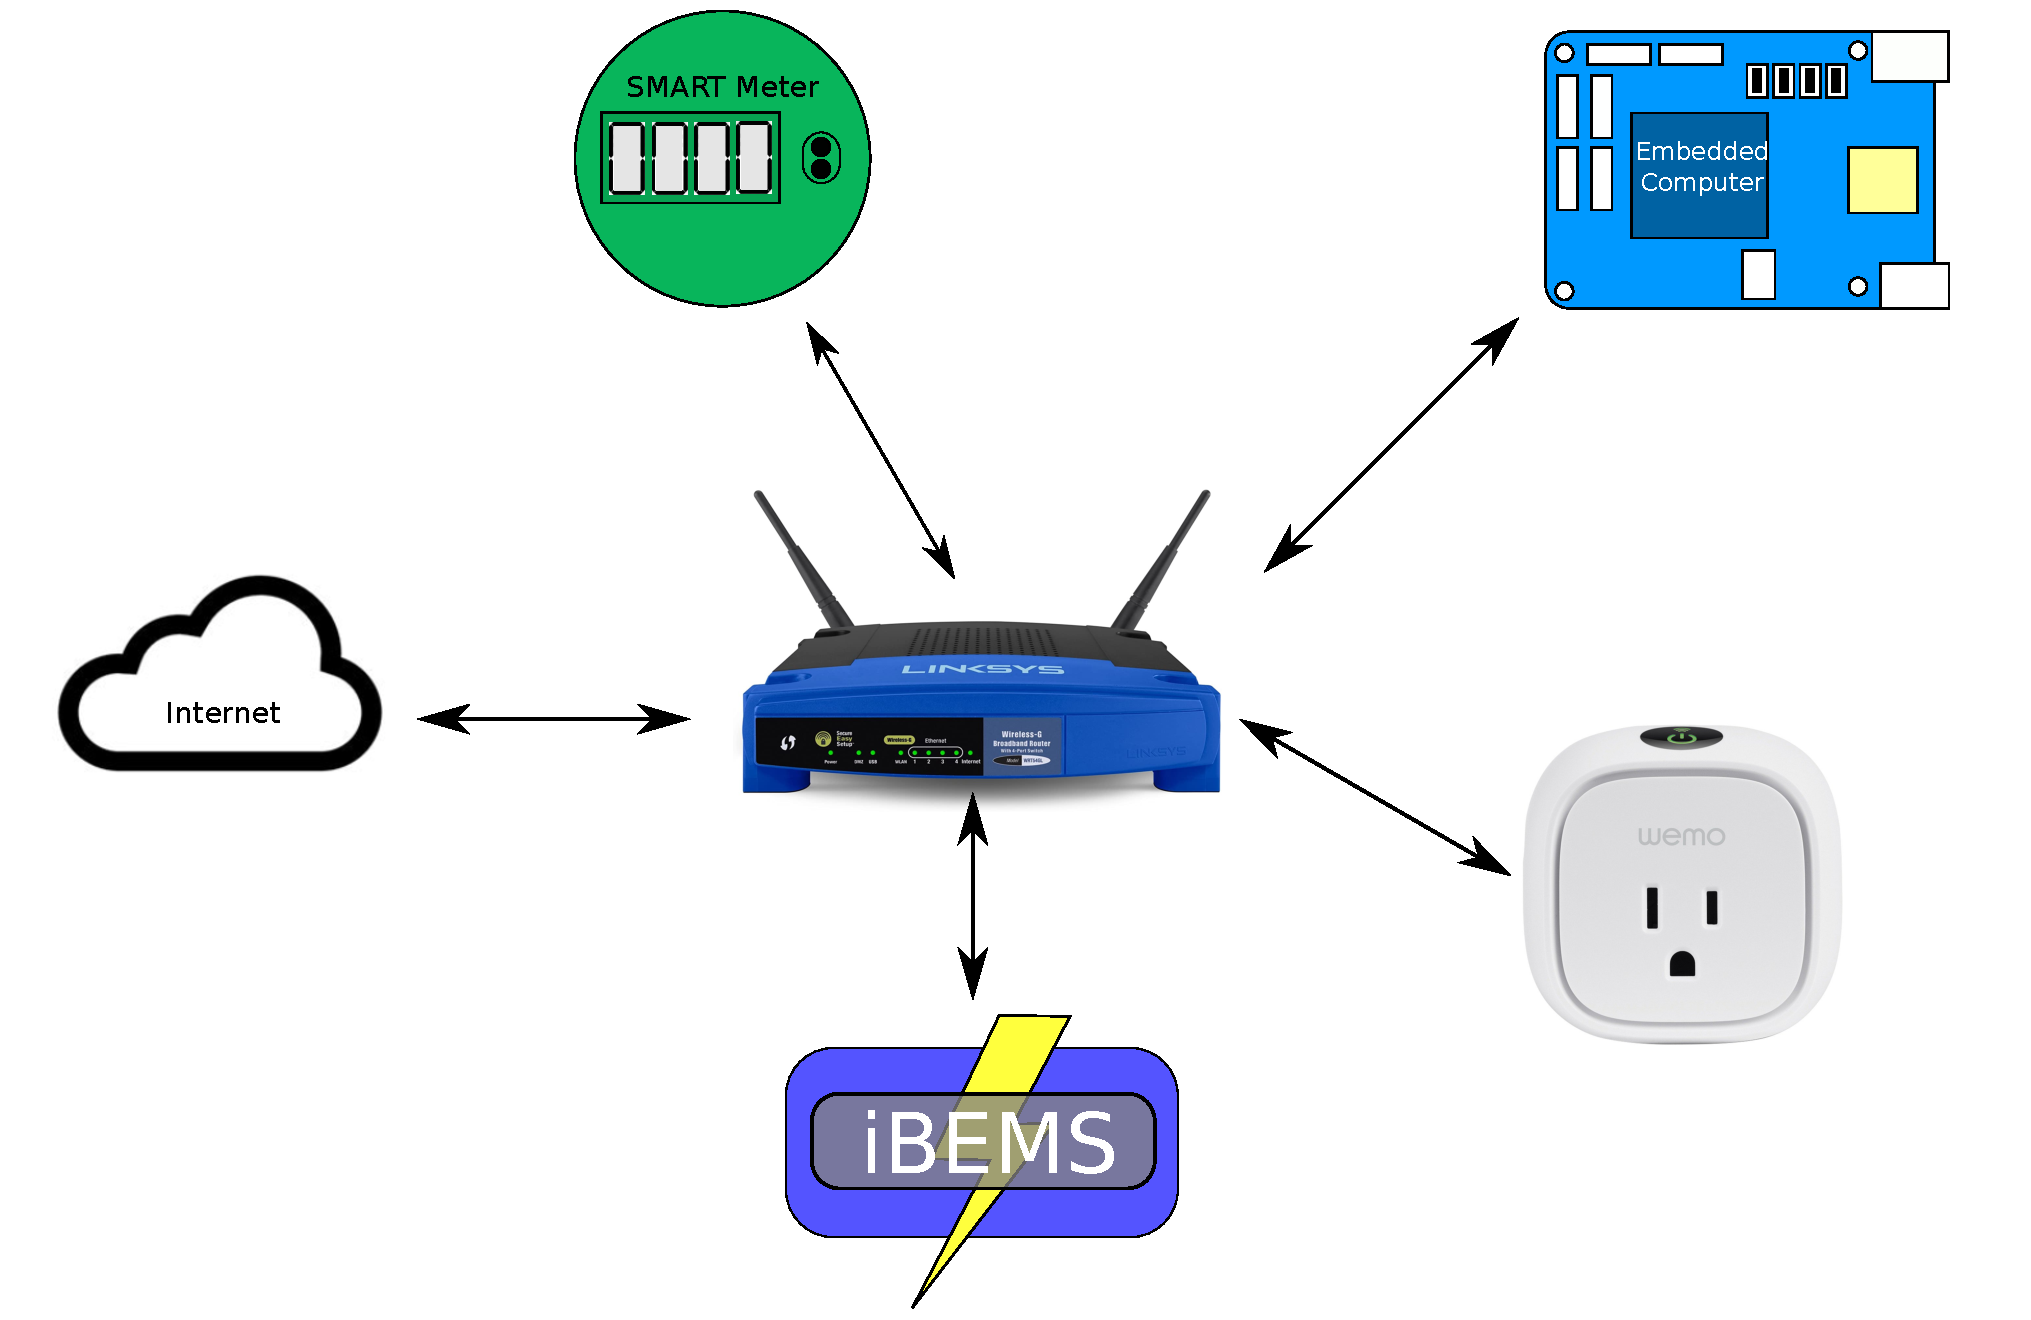
\includegraphics[scale=0.15]{figs/overallConnectionDiagram.pdf}
  \caption{High-level architecture of the proposed iBEMS.}
  \label{fig:highLevelArchitecture}
\end{figure}
%
These devices are the WeMo Insight Switch and an embedded computer known as the Beaglebone
Blue.  The core is also able to
connect the internet to download weather data for a local city through
OpenWeatherMap. Fig.~\ref{fig:functional_bd} gives the lower level functional block diagram of the system
architecture. %
%
\begin{figure}[htbp]
  \centering
  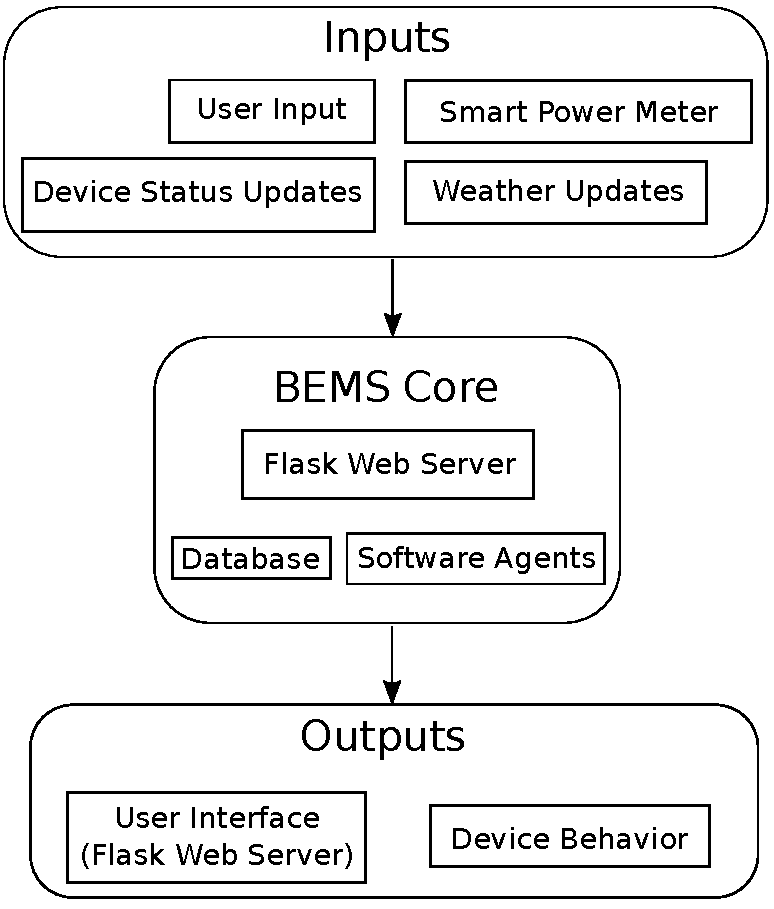
\includegraphics[scale=0.15]{figs/functionalBlockDiagram.pdf}
  \caption{Functional Block Diagram}
  \label{fig:functional_bd}
\end{figure}
%
The inputs include the user input through the web server, the device status
updates (On/Off, power usage, etc...) and the weather data. The iBEMS Core
itself consists of a Flask Web Server, 2 databases (Apache Cassandra and
SQLite), and 3 software agents (Discovery, Control, and Scheduling).


The Flask web server is built using a Python web framework titled Flask which
allows programmers to develop a dynamic web server capable of rendering data to
HTML pages. The benefit of this framework over other Python web frameworks like
Django is the large amount of customization available. For example, the
developers can create a completely custom user login system. For now, the server
is capable of being accessed only on the server computer running Ubuntu Linux.
In the future, support could be added to allow any user on the LAN to access the
web server. Other web frameworks use object relational mapping directly to
access the relevant databases. However, the current iBEMS uses direct queries with both
SQLite and the Cassandra query language to query the databases. We used
2 different databases to store information on. The Apache Cassandra database was
better suited for the time series data such as device status and power usage.
This database was therefore utilized a lot by the Control and Scheduling Agents.
The SQLite database hold parameters that do not change over time like device
ID's, IP addresses, and MAC addresses which made it amendable to the processes
in the Discovery Agent. The first agent that is
used by the iBEMS Core on startup is the discovery agent. It is responsible for
reaching out on the network and finding all devices that the iBEMS Core has
support for. This process involves retrieving the following parameters: IP
address, Port number, MAC address, Manufacturer, Name, and API. Once all
available devices are connected, the Control agent is used to change the status
of each device and collect power usage data in real time. Finally, the
scheduling will take input from the user and place the corresponding scheduling
periods in the Apache Cassandra database. Then, a thread is created to poll the
current device status at regular intervals and update the status if it does not
match the defined status in the Apache Cassandra database.


Fig.~\ref{fig:systemComponentInterconnection} provides an explanation of how
the components of the system interact with each other. %
%
\begin{figure}
  \centering
  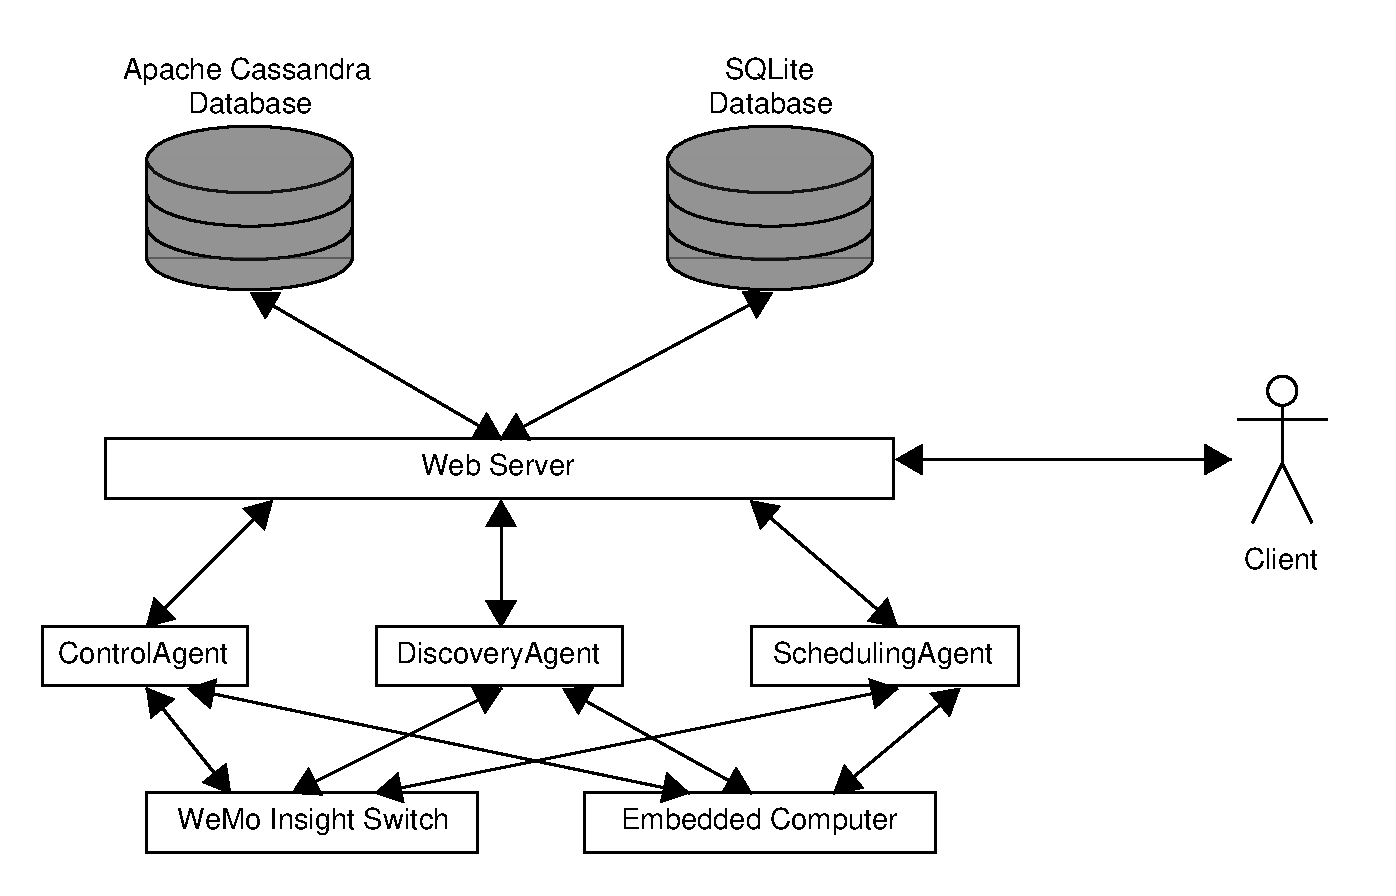
\includegraphics[scale=0.15]{figs/overallDiagram.pdf}
  \caption{Interconnection between system components}
  \label{fig:systemComponentInterconnection}
\end{figure}
%
The Apache Cassandra database and SQLite database are accessible from the web server, control agent, discovery agent, and scheduling agent. The web server queries the time series database and metadata database for vastly different purposes. Power plotting requires querying the Apache Cassandra database. To distinguish between the different devices on the front end, the metadata database is used. The agents utilize the Apache Cassandra database for storing and extracting time-series data. The agents use the metadata database to distinguish between different devices. 

\section{Software Implementation}
\label{sec:SoftwareImplementation}

To provide the ability to recognize and control devices at any moment, three agents are used. All three agents communicate with each other and the web server using the Zero MQ asynchronous messaging library. Essentially, this library works as a way to implement inter process communication without a message
broker\footnote{\href{https://zeromq.org/}{https://zeromq.org/}}. In other words, different processes are able to communicate with each
other without any central bus. This is convenient as fewer processes are needed for the system to function. Lowering the number of overall processes lowers the
RAM and CPU usage of the software. The library is ported to many different programming languages; however we are using the Python port titled Pyzmq to
implement in our code base.
%
\begin{figure}[htbp]
    \centering
    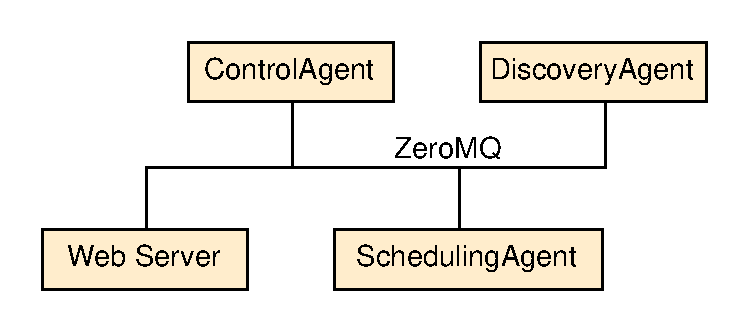
\includegraphics[width=0.4\textwidth]{figs/agents/pubSubAgents.pdf}
    \caption{Publish Subscribe Communication using ZeroMQ}
    \label{fig:pubSubAgents}
\end{figure}

More specifically, the publish subscribe model of communication is used where
each agent communicates via a socket where each socket responds to a specific
topic. The topics and port numbers are listed below along with their
corresponding agents in Table~\ref{tab:pubsubspecs}. %
%
\begin{table}[htbp]
    \centering
    \begin{tabular}{|c|c|c|}
        \hline
        Agent & Topic & Port Number\\
        \hline
        Discovery Agent & "discovery" & 5556\\
        Scheduling Agent & "scheduling" & 5556\\
        Control Agent & "control" & 5556\\
        \hline
    \end{tabular}
    \caption{Publish/Subscribe Communication Specifications}
    \label{tab:pubsubspecs}
\end{table}
The agents contained in the software are associated with a Python class of the
same name. Each class is instantiated and run with specifications declared in
Table~\ref{tab:pubsubspecs}. 

The flow chart of method \texttt{setDeviceStatus} defined in the \texttt{ControlAgent} class is shown in
Figure~\ref{fig:setDeviceStatus}. The purpose of this method is to set the
status of the desired device. When the method is called, the data dictionary is
obtained which contains the device ID. With this device ID, the API type can be
determined using the SQLite database. Subsequently, the appropriate device API
module can be imported. If the power state exists as a key in the device data
dictionary, the power state of the WeMo Insight Switch will be set as ON or OFF.
If the duty cycle key exists, the duty cycle of the single board computer motor
drivers is set. If the shutdown key is set, the single board computer is
shutdown. In order to reconnect to the single board computer, the board must be
started and receiver program ran. If necessary, the device must be reconnected
to the WiFi network. %

\begin{figure}[htbp]
    \centering
    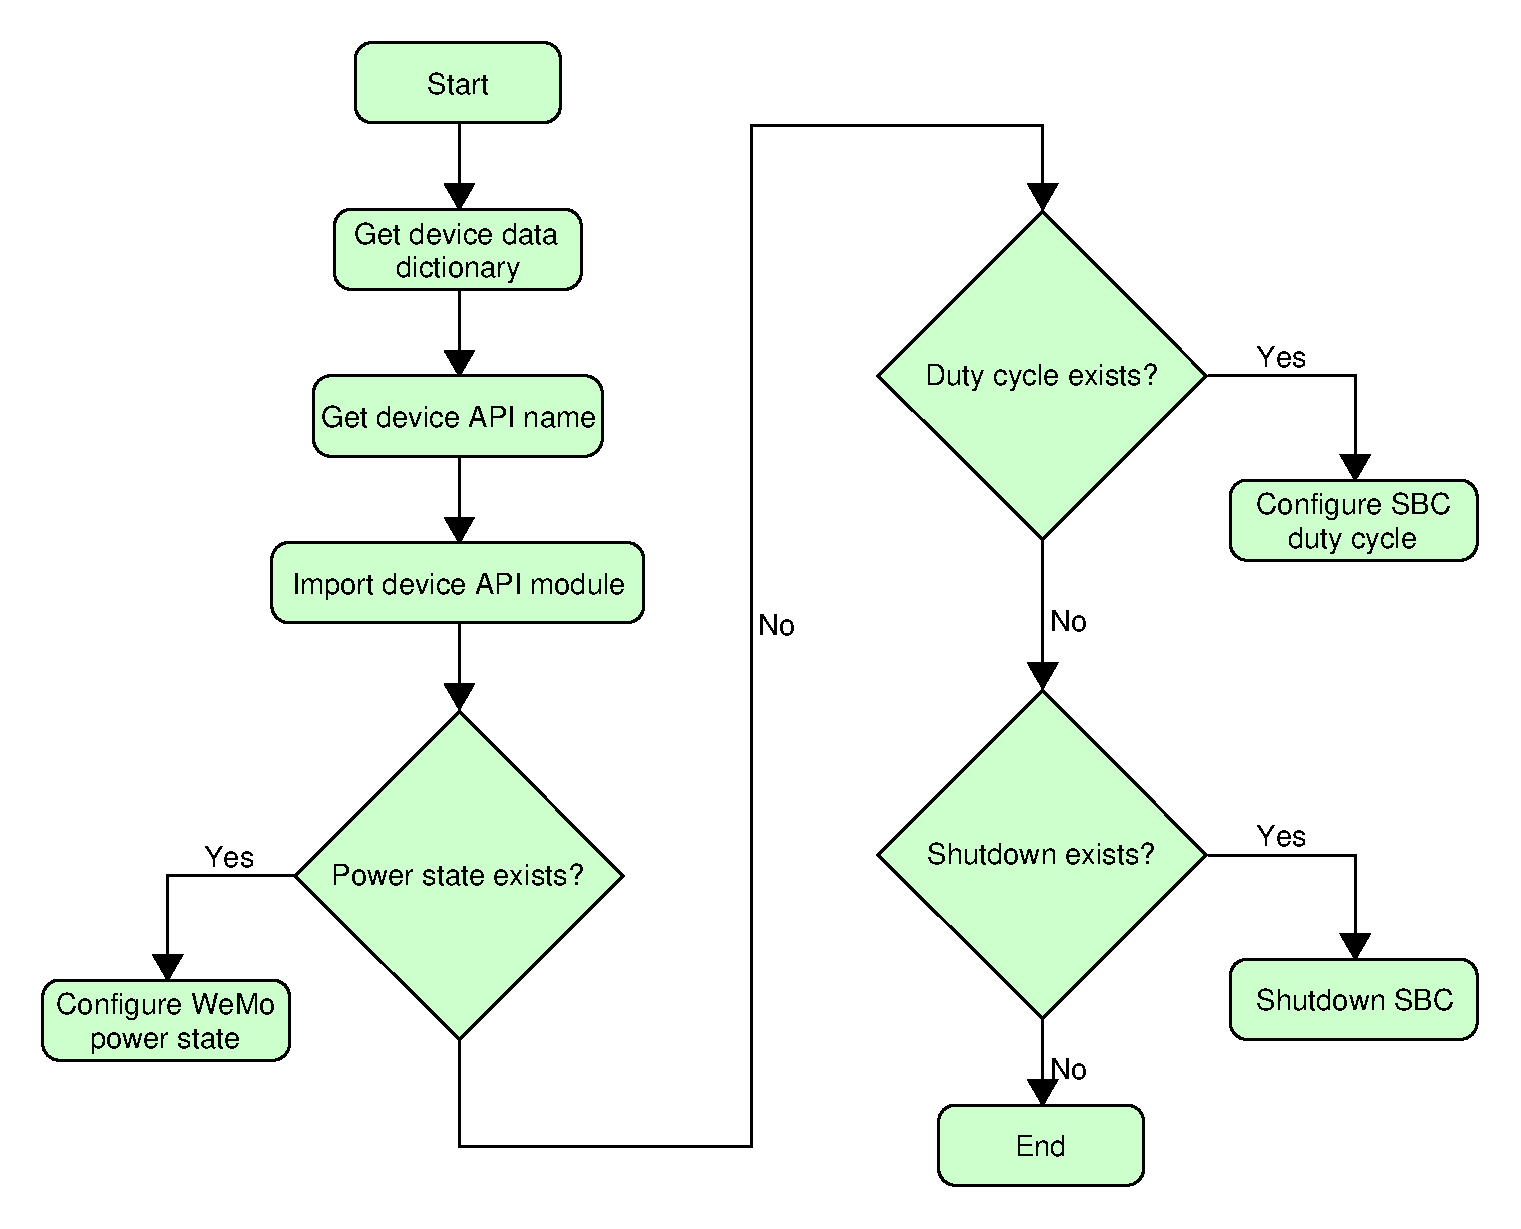
\includegraphics[scale=0.2]{figs/agents/setDeviceStatus.pdf}
    \caption{setDeviceStatus Flow Chart}
    \label{fig:setDeviceStatus}
\end{figure}

To obtain necessary data quantities from the device, the
\texttt{getDeviceStatus} method defined in \texttt{ControlAgent}, defined in Figure~\ref{fig:getDeviceStatus}, is called. Once the proper data parameters are
obtained, the \texttt{getState} function defined in the devices API module can
be called with the data parameters such as power state and
status. Once the agent has finished sending these to the device, a request is
sent to the web server to inform the server that it completed searching for the
required device data. %
%
\begin{figure}[htbp]
    \centering
    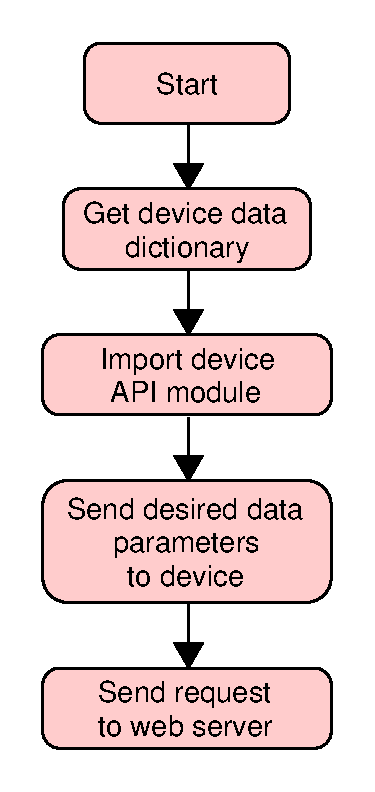
\includegraphics[scale=0.3]{figs/agents/getDeviceStatus.pdf}
    \caption{getDeviceStatus Flow Chart}
    \label{fig:getDeviceStatus}
\end{figure}

Every device connected to iBEMS will have a thread associated with it started from the control agent. This thread will run the \texttt{periodicQueryBehavior} method defined in \texttt{ControlAgent} to periodically query for device data and store in the corresponding Cassandra database table. A user specified delay is placed in the class's module to prevent the thread from overwhelming the system.

\begin{figure}[htbp]
    \centering
    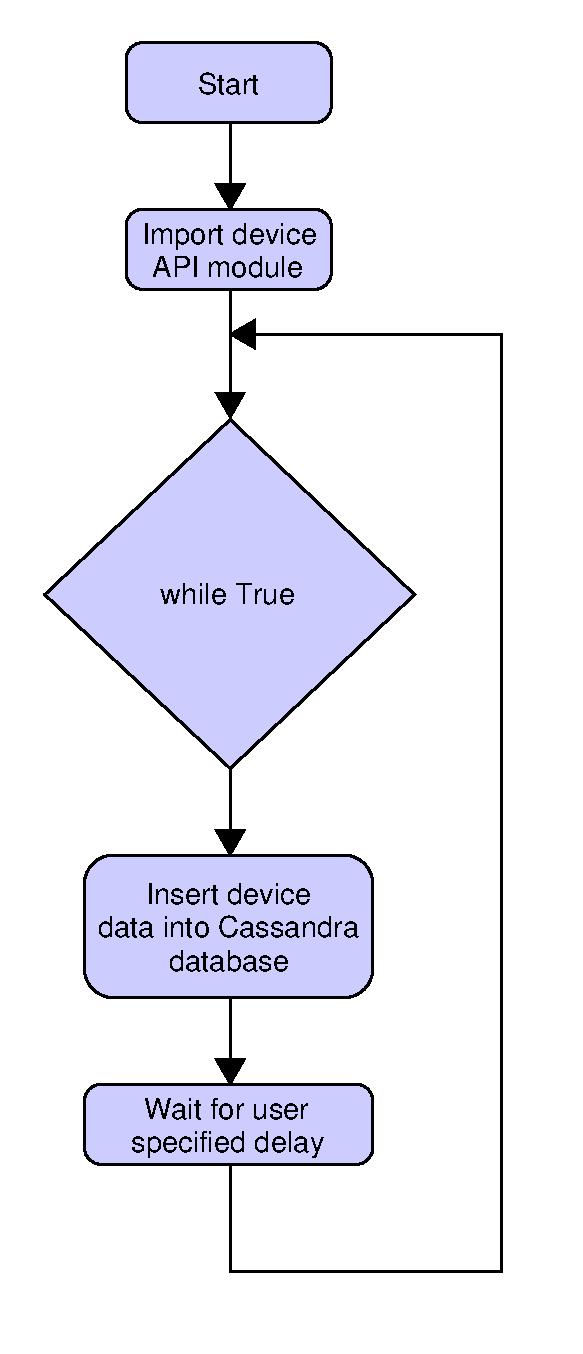
\includegraphics[scale=0.3]{figs/agents/periodicQueryBehavior.pdf}
    \caption{periodicQueryBehavior Flow Chart}
    \label{fig:periodicQueryBehavior}
\end{figure}

To reduce latency, the device status is retrieved directly from the API module in the \texttt{periodicQueryBehavior} method defined in \texttt{ControlAgent} rather than calling \texttt{getDeviceStatus} as this prevents the API from being imported unnecessarily.

The scheduling agent is able to update the device status of each device dependent on whether a schedule is set for the specific time period and day. One of the methods that is called, \texttt{updateScheduleFromServer} is invoked when the user presses the \say{Update Schedule} button from the UI on the scheduling page. A flow chart of this method is shown in Figure~\ref{fig:updateScheduleFromServer}. When this method is called the desired schedule is loaded in as a dictionary and parsed to extract the necessary periods and given day. First the times are stored in military time in the database for more convenient storage and parsing later on. Then, a table is created in the Apache Cassandra database where the device ID and day are embedded in the name. The previous table's data is destroyed to ensure there are no errors regarding overlapping schedules. Lastly, all the scheduling periods extracted from the dictionary are stored as rows in the table. 
\begin{figure}[htbp]
    \centering
    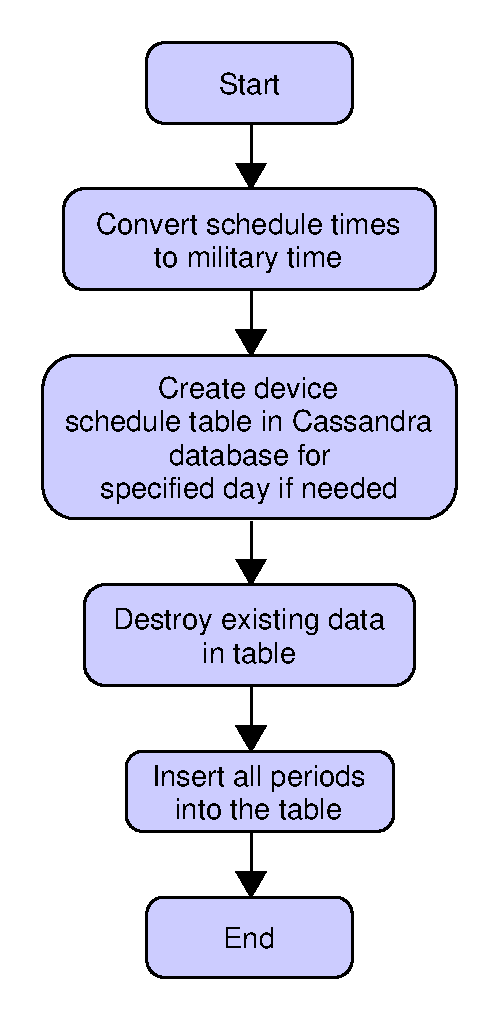
\includegraphics[scale=0.2]{figs/agents/updateScheduleFromServer.pdf}
    \caption{updateScheduleFromServer Flow Chart}
    \label{fig:updateScheduleFromServer}
\end{figure}
A second method that is run inside each device thread is \texttt{periodicDeviceUpdateMethod}, defined in Figure~\ref{fig:periodicDeviceUpdateMethod}, which is started when the discovery agent sets the discovered device to active. By first loading the device's API name, the scheduling agent can begin checking for scheduling periods inside an infinite loop. The status dictionary is queried from the Cassandra database and loaded into a dictionary. All these scheduling periods are looped over for the current day while constantly checking whether the current time in seconds is within the starting and ending time. A conversion of both starting and ending time to seconds is necessary as it is challenging to work with these quantities in standard and military time when comparing times. If the current time does lie inside the scheduling period, the device's state is set dependent on the API. 
\begin{figure}[htbp]
    \centering
    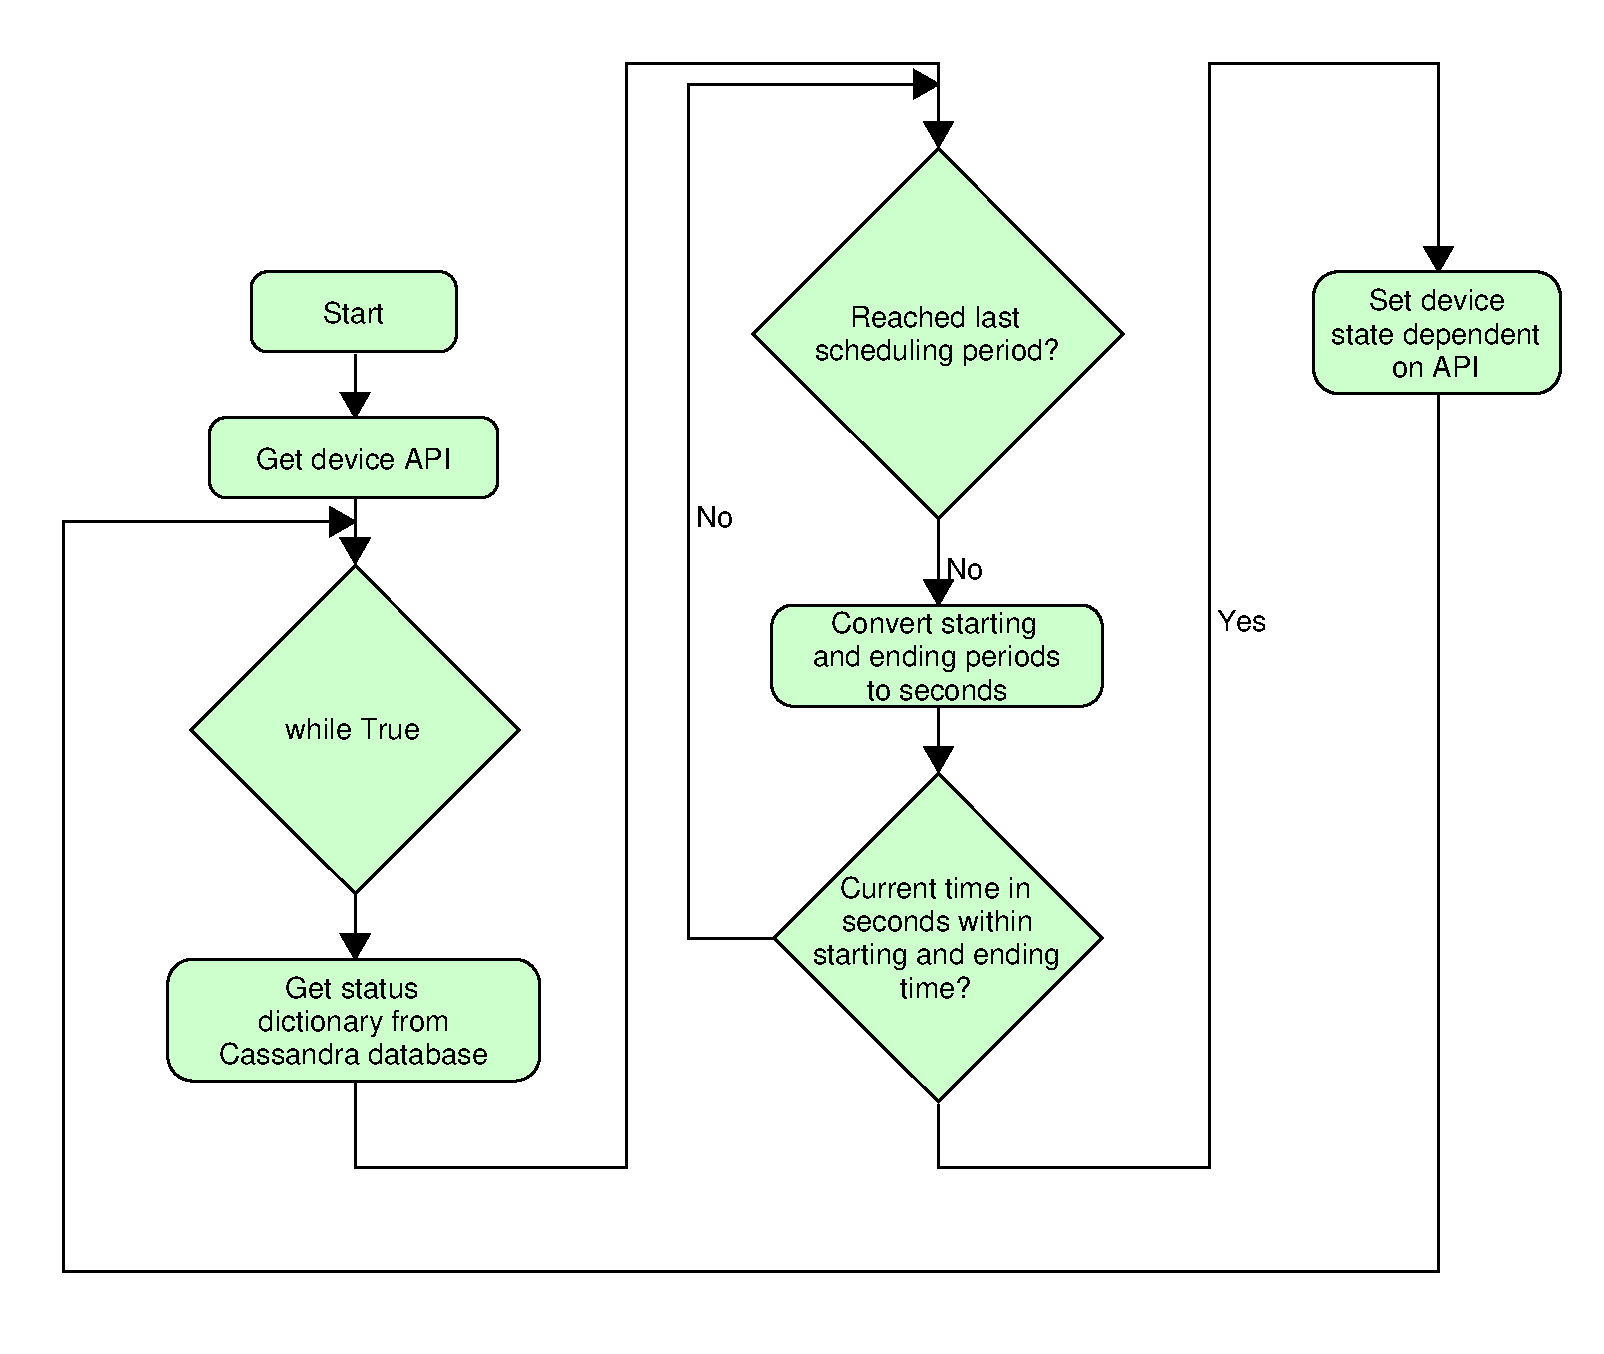
\includegraphics[scale=0.2]{figs/agents/periodicDeviceUpdateMethod.pdf}
    \caption{periodicDeviceUpdateMethod Flow Chart}
    \label{fig:periodicDeviceUpdateMethod}
\end{figure}

\begin{figure}[htbp]
    \centering
    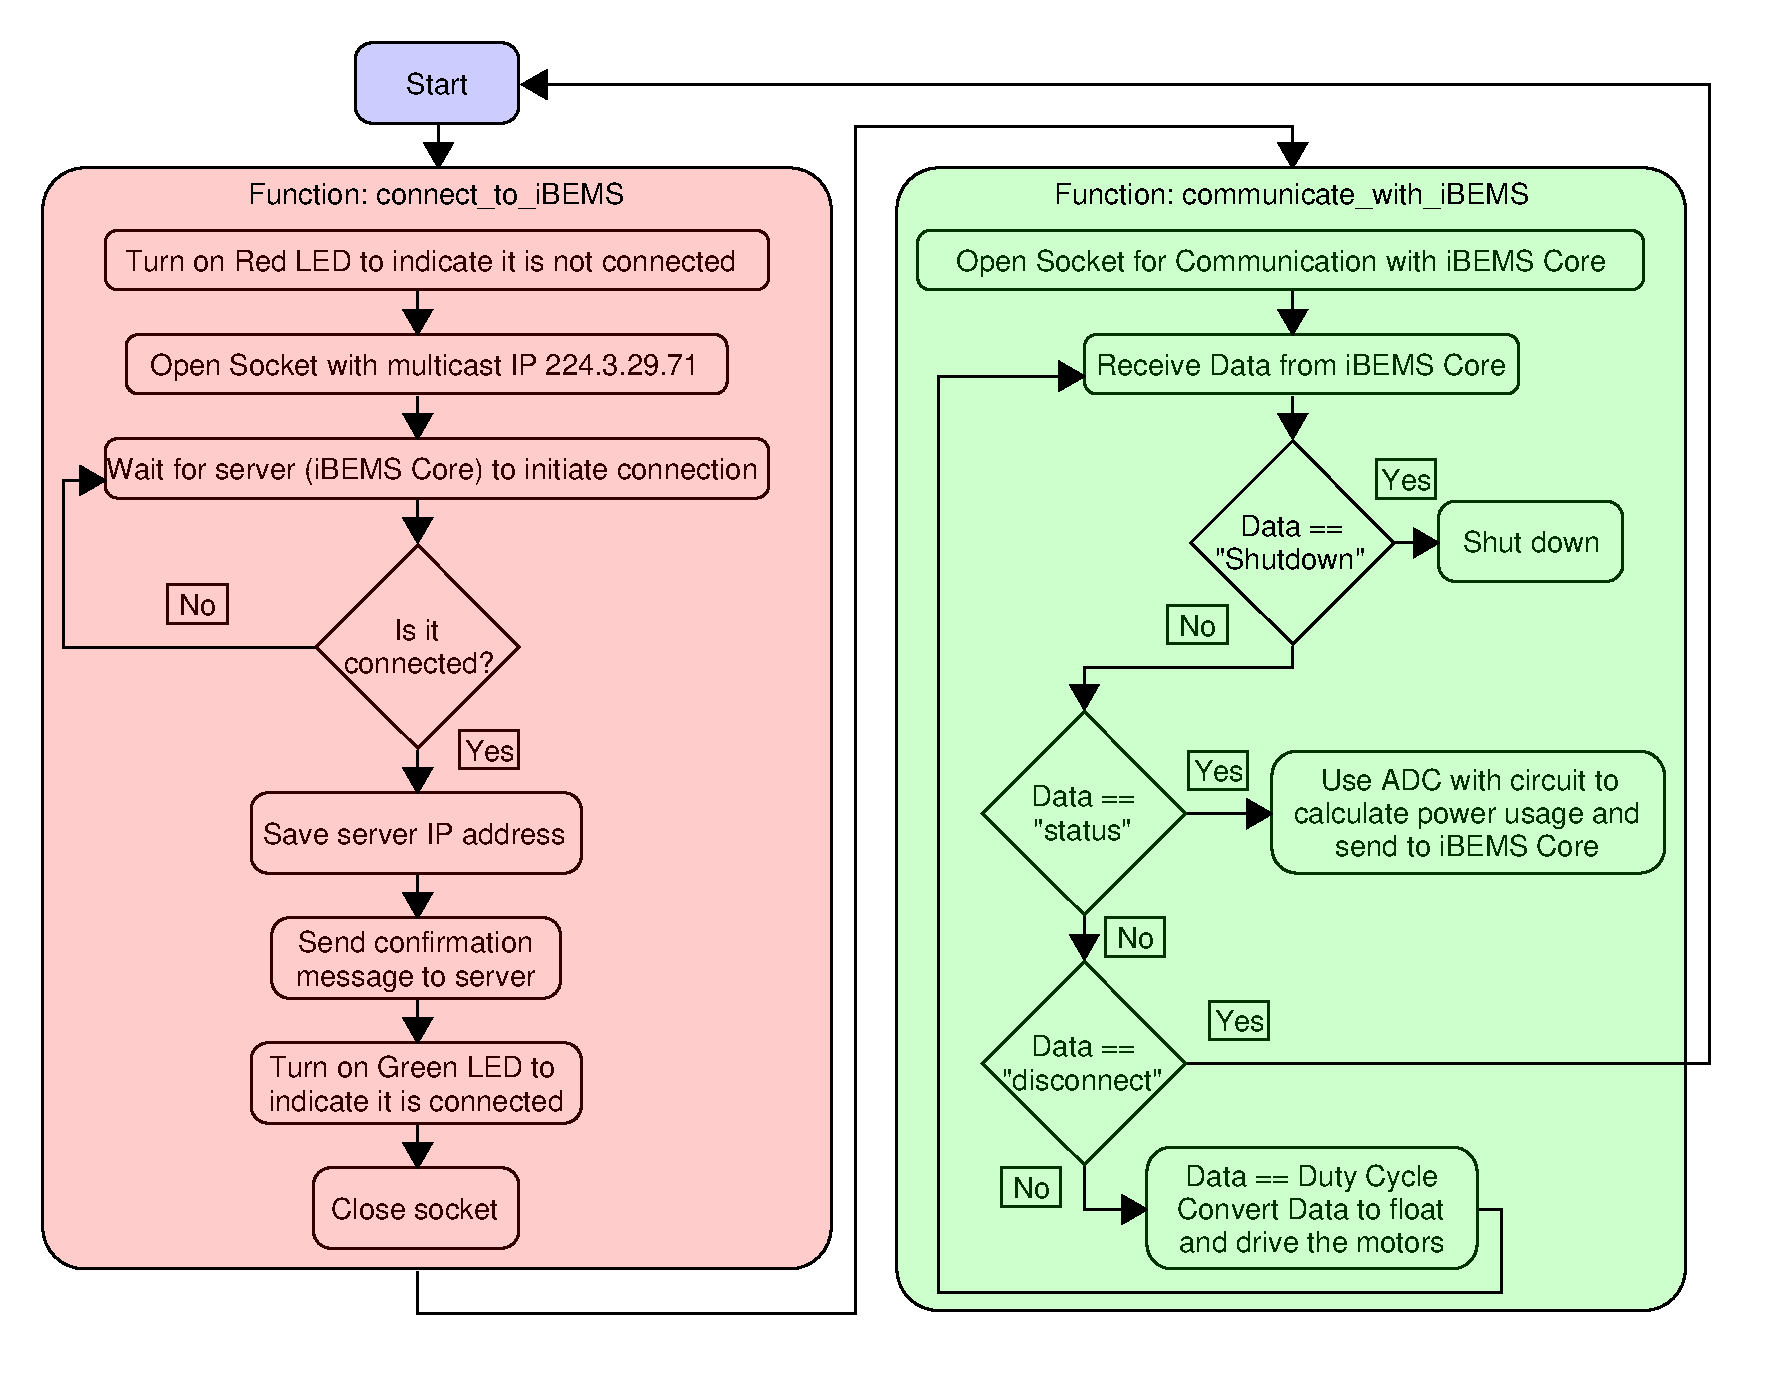
\includegraphics[scale=0.2]{figs/beaglebone/Beaglebone_Receiver_Diagram.pdf}
    \caption{Receiver Running on Embedded Computer}
    \label{fig:Beaglebone_Receiver_Diagram}
\end{figure}

The embedded computer needed some software to be able to connect to and communicate with the iBEMS Core. To achieve this, a program consisting of 2 functions for connecting and communicating is used.
\medbreak
The first of these functions is \texttt{connect\_to\_iBEMS}. This function first turns on the red LED on the embedded computer to indicate it is not yet connected. Then it creates a socket using a multicast IP address that the corresponding API in the iBEMS core will be looking for. Once the socket is created, the embedded computer will enter a loop and wait for the iBEMS core to make the initial connection. When that connection is made, it will exit the loop, save the IP address of the iBEMS core, send a confirmation message, then turn on the green LED before closing the multicast socket.
\medbreak
The second function, \texttt{communicate\_with\_iBEMS} will open another socket but with the IP address of the iBEMS core found in \texttt{connect\_to\_iBEMS}. It will then enter an indefinite loop to continually receive data from the iBEMS core. There are 4 different messages that the iBEMS core sends to the embedded computer. First, it will check if the iBEMS core is telling it to shut down with the command \say{Shutdown}. If so, the embedded computer will immediately shut down. Second, if the data sent by iBEMS is \say{status}, the embedded computer will take a reading from the power measurement circuit. In case the user decides to shut down the iBEMS core without turning off the embedded computer, another message \say{disconnect} will be sent in which case the embedded computer will exit \texttt{communicate\_with\_iBEMS} and start the entire program over again. Finally, if iBEMS is not sending any of the above options, it means that the user is sending a new duty cycle to drive the motors with. Since iBEMS only sends messages with the string data type, this has to be converted to a float in order to call the motor driver function. 

\section{Experimental Results}
\label{sec:iBEMS-Experimental Results}
The system was tested with a working prototype, in which the first mode is the startup menu:

\begin{figure}[htbp]
    \centering
    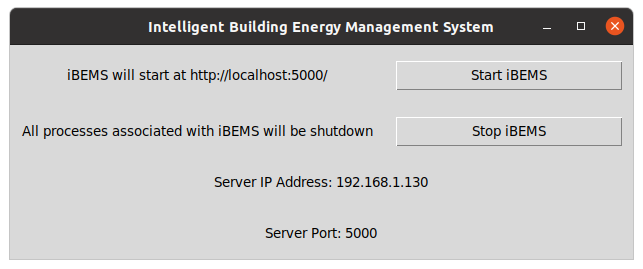
\includegraphics[scale=0.2]{figs/GUI/BEMS_GUI_Linux.png}
    \caption{Desktop GUI}
    \label{fig:desktopgui}
\end{figure}

\noindent
Here, the user will simply click the \say{Start iBEMS} button to launch the web server and agents. When the user is finished, all agents and the web server can be shut down by clicking \say{Stop iBEMS}. In case the user accidentally clicks the \say{Start iBEMS} button while iBEMS is already running, then the following error message will appear:

\begin{figure}[htbp]
    \centering
    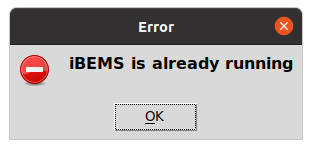
\includegraphics[scale=0.3]{figs/GUI/BEMS_GUI_Linux_Warning.png}
    \caption{Popup Error}
    \label{fig:popuperror}
\end{figure}

\noindent
After launching iBEMS, the web browser will open and the user will be presented with the login page:

\begin{figure}[htbp]
    \centering
    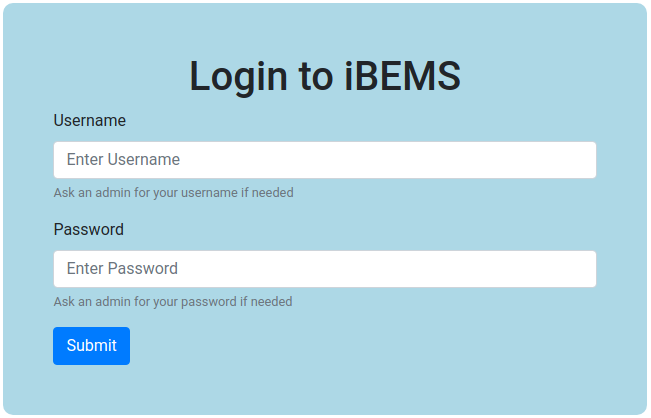
\includegraphics[scale=0.2]{figs/webServer/Login.png}
    \caption{Login Page}
    \label{fig:Home_screen}
\end{figure}

\noindent
where the user can enter in their username and password. Currently, iBEMS does not have a robust user login. It actually just has 1 username and password that is defined in the code. When the user enters the valid username and password, the home page will load automatically, where the weather data can be seen:

\begin{figure}[htbp]
    \centering
    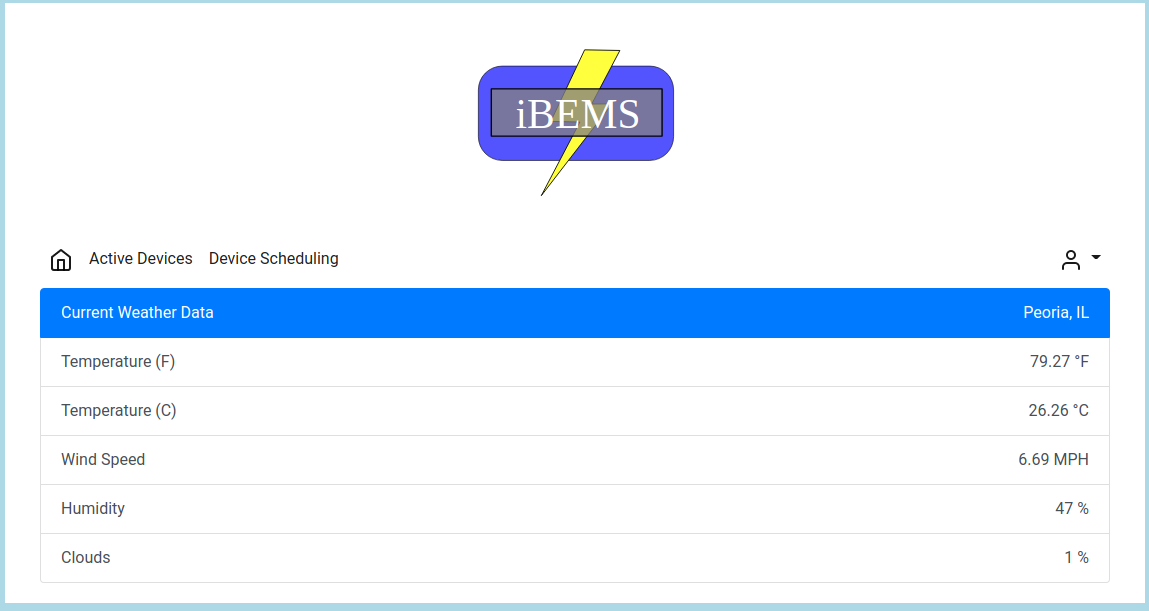
\includegraphics[scale=0.2]{figs/webServer/Home_screen.png}
    \caption{Home Page}
    \label{fig:Home_screen}
\end{figure}

The home screen (mode 2) does not have any interactive functionality other than to load another page by selecting one on the navigation bar.

\begin{figure}[htbp]
    \centering
    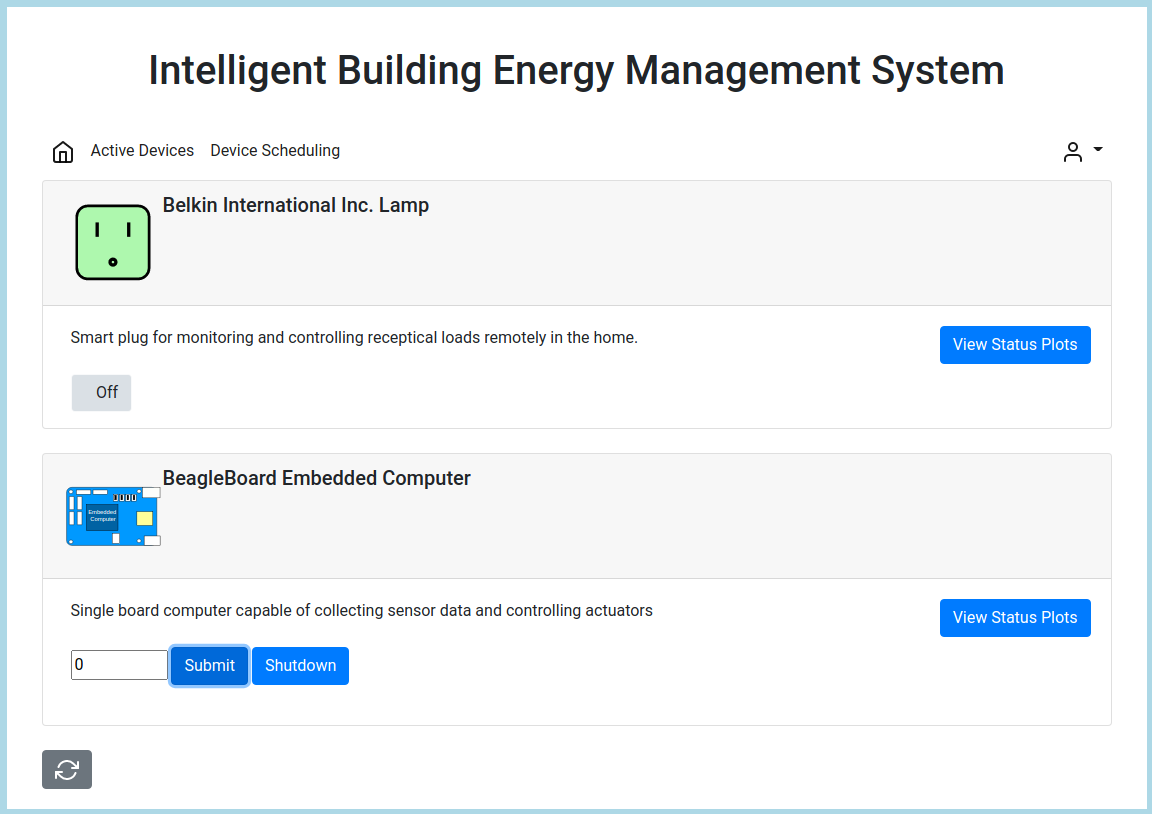
\includegraphics[scale=0.2]{figs/webServer/ActiveDevices_screen.png}
    \caption{Active Devices Page}
    \label{fig:active_devices}
\end{figure}

Figure~\ref{fig:active_devices} shows the active devices page (mode 3) which is loaded upon clicking \say{Active Devices} in the navigation bar. Here, all the connected devices are shown in order of when they connected to iBEMS. As mentioned previously, control of the WeMo Insight Switch is limited to turning it on and off while the embedded computer's motor speed can be controlled by submitting different duty cycles. Additionally, the embedded computer can be completely turned off by clicking the \say{Shutdown} button. Both supported devices also log their power usage at regular intervals. A plot of these power usage data points can be viewed by clicking \say{View Status Plots}.

\begin{figure}[htbp]
    \centering
    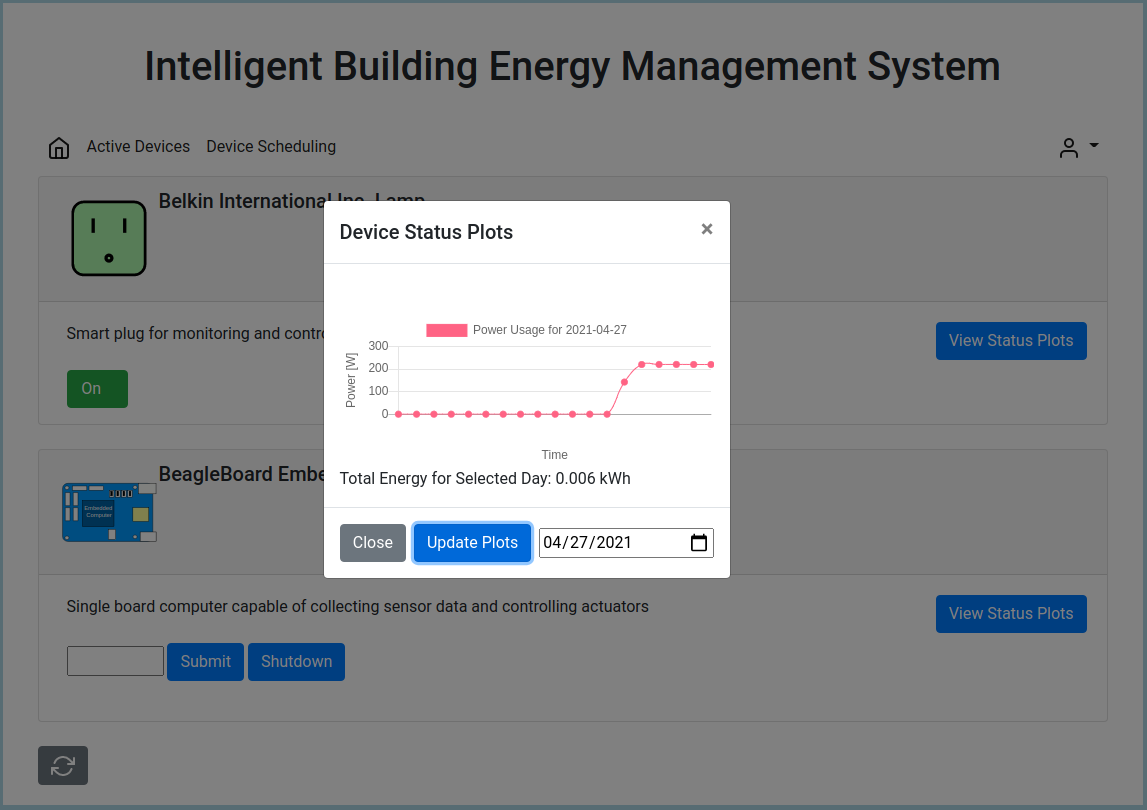
\includegraphics[scale=0.2]{figs/webServer/ActiveDevices_plot.png}
    \caption{Active Devices Plot}
    \label{fig:active_devices_plot}
\end{figure}

After clicking \say{View Status Plots}, a modal will pop up for the user to further interact with. By default, power usage data points for the current day are loaded at first, but another day can be selected by clicking on the calendar icon in the lower right corner. The plot is then updated by clicking \say{Update Plots}. This is done by collecting data from the Apache Cassandra database and simply plotting all the points found for the specified day. Underneath the plot, the total energy consumed for the specified day is displayed. That total energy is found using the trapezoid method for integration on the plot.

\begin{figure}[htbp]
    \centering
    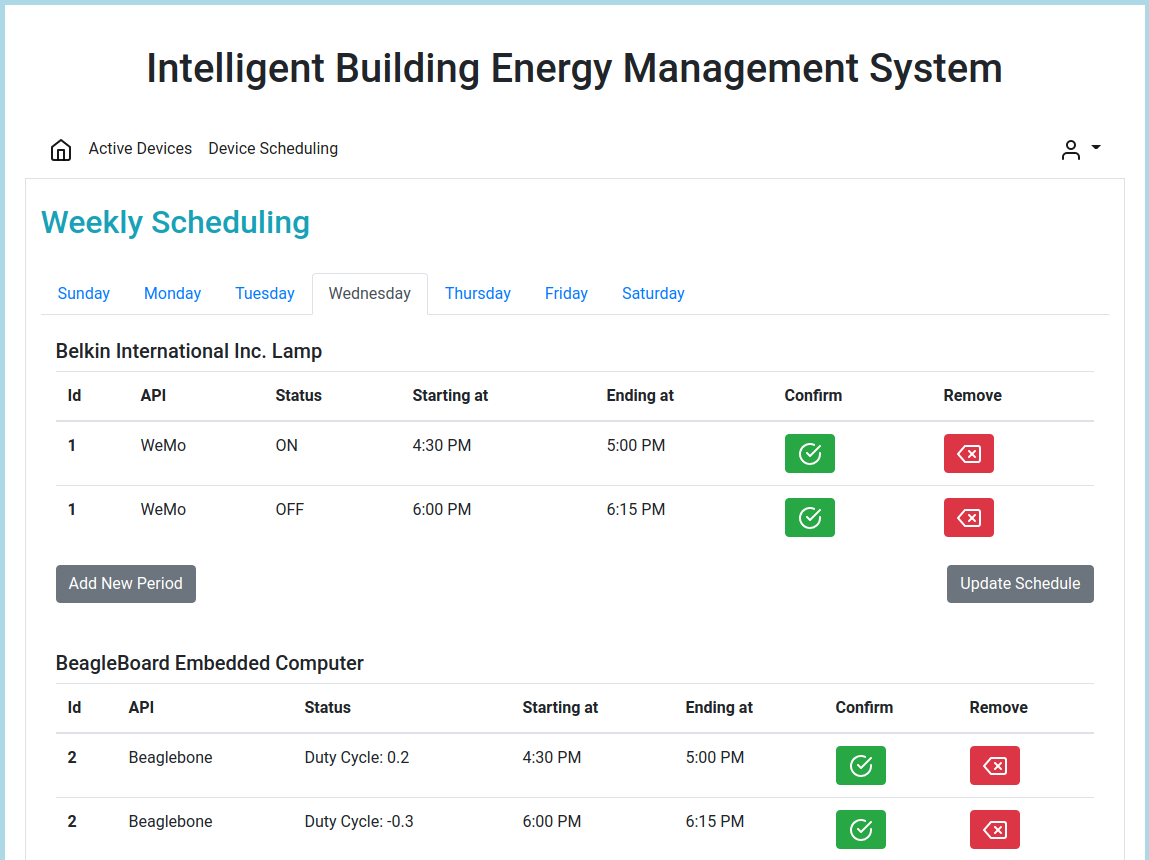
\includegraphics[scale=0.2]{figs/webServer/Applications_screen.png}
    \caption{Scheduling Page}
    \label{fig:schedulingl}
\end{figure}

Mode 4, or the scheduling page, can be loaded by clicking the \say{Device Scheduling} button in the navigation bar. Much like the active devices page, each connected device is listed in order of when they connected to iBEMS. Instead of directly controlling the devices, the user can enter in time periods when they want each device to maintain a specified status. For example, the WeMo Insight Switch can be scheduled to be on from 5 to 8 P.M. on Fridays. Likewise, the embedded computer can be scheduled to maintain a duty cycle of 0.5 for the same time period every Friday. Scheduled times can be added with the \say{Add new Period} and deleted by clicking the red \say{X} by the corresponding time period.


\section{Conclusion and Future Work}
\label{sec:conclusion}

We have presented a platform of an intelligent building energy management system,
which is open source, and easy-to-use. It is also developed using a modular, agent-based code base. Being open source makes it freely available to anyone who has the supported devices and wants to begin managing their home energy usage. The simple interface is easy to figure out for less tech-savvy users and the modular code base makes this system relatively easy for others to continue development. Despite its advantages, potential users are to be aware of the rather obvious disadvantages at this point. A typical commercial building energy management system will include many more features like predicting future energy use and supporting more devices.

One of the main ways to improve the software is to refactor the user interface as the current interface is fairly primitive. Adding elements like collapsible drop down menus and a collapsible side bar would make the interface more professional and user-friendly. To improve the overall reliability and speed of the software, a better agent communication protocol could be researched and implemented. Many problems are visible with the use of ZeroMQ as exceptions are thrown occasionally when device status updates are sent in quick succession to the control agent. Potentially, there exists a better solution than publish-subscribe. One of the major issues with the software is lack of device data persistence across system restarts. Developers in the future could help alleviate this problem by refactoring the device storage system in the Cassandra database.

\bibliographystyle{IEEEtran}
\bibliography{bib/references.bib}

\end{document}
